\begin{frame}{Examle: Congestion Control}
    Property: at most one packet can reach $e$
    \begin{center}
        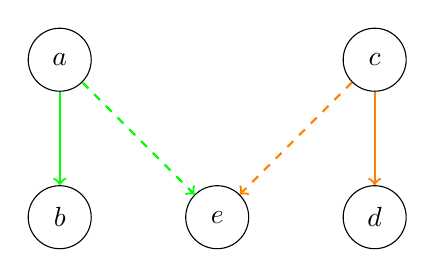
\begin{tikzpicture}[node distance={20mm},main/.style = {draw, circle,minimum size=8mm}]
            \node[main] (a)  {$a$};
            \node[main] (b) [below of=a]  {$b$};
            \node[main] (e) [right of=b] {$e$};
            \node[main] (d)  [right of=e] {$d$};
            \node[main] (c) [above of=d] {$c$};
            \draw [->,green,thick] (a) -- (b);
            \draw [->,orange,thick] (c) -- (d);
            \draw [->,green,thick,dashed] (a) -- (e);
            \draw [->,orange,thick,dashed] (c) -- (e);
        \end{tikzpicture}
    \end{center}
    \begin{equation*}
        \begin{aligned}[c]
            P   & = p!1                             \\
            Q   & = q!1                             \\
            N   & = F^2 \oplus p?1;N_p \oplus q?1;N_q \\
            N_p & = F_p^2 \oplus q?1;F_{pq}^2          \\
            N_q & = F_q^2 \oplus p?1;F_{pq}^2           \\
            F   & = ab \oplus cd                    \\
        \end{aligned}
        \qquad
        \begin{aligned}[c]
            F_p         & = ae \oplus cd         \\
            F_q         & = ce \oplus ab         \\
            F_{pq}      & = ae \oplus ce         \\
            SDN         & = \delta_{\mathcal{L}}
            (N \parallel P \parallel Q)          \\
            \mathcal{L} & = \s{p!1,p?1,q!1,q?1}
        \end{aligned}
    \end{equation*}
\end{frame}

\begin{frame}{Examle: Congestion Control}
    Property: at most one packet can reach $e$
    \begin{align*}
        \f{PV} & = \exists c,c' \in \mathcal{F}(ES(\vec v)).
        \exists e \in c,e' \in c'. l(e) = ae \wedge l(e') = ce
    \end{align*}
    Here we can declare $C(p_1,q_1) = \F$ as a cause using the 
    witness $(C(p_2,q_2),\T,\T)$
    \begin{center}
        \begin{tikzpicture}
            \crd{0}{0}{$\emptyset$}
            \crd[left]{-2}{1}{$\s{p_1}$}
            \crd[left]{-2}{2}{$\s{p_1,q_1}$}
            \crd[above]{-1}{3}{$\s{p_1,q_1,ae_1}$}
            \crd[left]{-3}{3}{$\s{p_1,q_1,ce_1}$}
            \crd[right]{2}{1}{$\s{q_2}$}
            \crd[right]{2}{2}{$\s{p_2,q_2}$}
            \crd[above]{1}{3}{$\s{p_2,q_2,ae_2}$}
            \crd[right]{3}{3}{$\s{p_2,q_2,ce_2}$}
            \draw [ultra thick] (-2,1) -- (-2,2);
            \draw [ultra thick] (-2,2) -- (-1,3);
            \draw [ultra thick] (-2,2) -- (-3,3);
            \draw [ultra thick] (0,0) -- (2,1);
            \draw [ultra thick] (0,0) -- (-2,1);
            \draw [ultra thick] (2,1) -- (2,2);
            \draw [ultra thick] (2,2) -- (1,3);
            \draw [ultra thick] (2,2) -- (3,3);
        \end{tikzpicture}
    \end{center}
\end{frame}
